\documentclass{article}
\usepackage[T1]{fontenc}
\usepackage{iclr2027_conference,times}
\usepackage{amsmath,amssymb,booktabs,graphicx,tabularx,xcolor,hyperref,microtype,etoolbox}
\hypersetup{colorlinks=true,linkcolor=blue!45!black,citecolor=blue!45!black,urlcolor=blue!45!black}
\makeatletter
\patchcmd{\@maketitle}{Under review as a conference paper at ICLR 2027}{Working draft -- 11 September 2026 -- not submitted}{}{\errmessage{Draft header patch failed}}
\patchcmd{\@maketitle}{Paper under double-blind review}{Evidence-grounded working draft}{}{\errmessage{Draft status patch failed}}
\makeatother
\newcommand{\asr}{\mathrm{ASR}}
\newcommand{\E}{\mathbb{E}}
\title{Addressable Memory Is Not a Security Boundary:\\Fine-Tuning Routes Triggered Behaviors into the Backbone}
\author{Anonymous authors}

\begin{document}
\maketitle

\begin{abstract}
Conditional-memory language models retrieve a small, deterministic set of
table rows for each token suffix. This makes a stored item inspectable and, in
principle, removable by deleting its addressed rows. We test whether this
architectural property controls where new behavior is stored during ordinary
fine-tuning. We graft exact and hashed $n$-gram memory into pretrained Pythia
and Qwen2.5 base models, poison fine-tuning with rare trigger--continuation
pairs, and intervene on the rows, the whole graft, and the backbone. Across four
model sizes and two tokenizer/architecture families, the behavior reaches
near-ceiling attack success while the graft is frozen. When the graft is
trainable, deleting the trigger's rows changes attack success by at most
$0.11$ percentage points at the upper confidence bound. Whole-component swaps
localize the learned behavior to the backbone: poisoned backbone plus clean
graft retains $99.65\%$/$99.49\%$ attack success, while poisoned graft plus
clean backbone yields zero. The null is not a broken intervention: direct
row-confined writes are removed by the identical deletion with $98.30$--$100\%$
effect across both families. Thus deterministic addressing provides a deletion
boundary only when the write path enforces storage in that boundary. Ordinary
fine-tuning can bypass it. We release preregistered protocols, raw per-prompt
predictions, component-level interventions, and full optimizer replays. Our
claim is limited to the tested Memory Grafting implementation, base models,
synthetic rare-string behaviors, and training recipe.
\end{abstract}

\section{Introduction}

Conditional memory has emerged as a way to add language-model capacity without
paying dense compute for every parameter. Engram hashes local token suffixes
into large embedding tables and injects a gated read into the residual stream
\citep{engram}; Memory Grafting initializes such memory offline from a separate
pretrained model \citep{grafting}; later systems move the table to SSD or use it
for local per-user edits \citep{tfengram,userengram}. Deterministic addressing
has an appealing security implication. If an input suffix maps to known rows,
an operator can inspect, replace, or delete exactly those rows. A local write
can even leave all other parameters bit-identical \citep{userengram}.

That implication silently joins two different claims: that a row is
addressable, and that gradient-based adaptation stores newly learned behavior
in that row. The first is architectural. The second is an optimization outcome.
A model with both dense weights and an addressable table can encode the same
mapping in either place, redundantly in both, or in interactions between them.
Deleting the nominal rows is meaningful only after locating the behavior.

We study this distinction with triggered continuation learning. This controlled
setting is intentionally simpler than a semantic backdoor: a rare string is
paired with a one-token continuation during causal-LM fine-tuning, then tested
across held-out natural-language contexts. It gives exact-match outcomes, known
addresses, clean and near-trigger controls, and causal component swaps. It also
connects conditional memory to a mature backdoor literature in which small
poison sets can install persistent conditional behavior \citep{badedit,sleeper}.

Our results identify a sharp boundary. Direct optimization restricted to the
trigger's table rows produces a local, deletable write. The same causal-LM
objective under ordinary parameter access takes a different route. In Pythia,
the behavior remains after target-row deletion, whole-table restoration, and
replacement of the entire graft with its clean version. Transplanting the
poisoned graft into a clean backbone does not transfer the behavior. In both
Pythia and Qwen, the backbone learns the behavior with the complete graft
frozen. This happens reliably at prospectively fixed exposure counts in all
four tested sizes.

We contribute:
\begin{itemize}
  \item a causal assay separating \emph{addressability} from \emph{storage},
  with target-row, random-row, benign-row, whole-table, whole-graft, and
  symmetric backbone/graft interventions;
  \item a verified negative result: a trainable deterministic memory does not
  preferentially absorb a newly fine-tuned trigger mapping under our ordinary
  recipe;
  \item positive controls showing that the same deletion removes behavior
  known to be row-confined in two model families; and
  \item cross-family evidence that an intact but frozen graft does not prevent
  the dense backbone from learning the mapping, including a low-exposure
  reliability failure that is preserved rather than selected away.
\end{itemize}

The conclusion is a design constraint, not a universal attack claim. A
conditional-memory system gains an auditable deletion boundary only if its
training interface constrains writes to that boundary or verifies where each
learned item landed.

\section{Conditional memory and the storage estimand}

At token position $t$, let $x_{\le t}$ be token IDs and let
$a_{n,h}(x_{\le t})$ deterministically map the final $n$-gram to a row of hash
head $h$. A graft retrieves row vectors, projects them, applies a
context-dependent scalar gate, and adds the result to the residual stream:
\begin{equation}
 r_t = \sum_{n,h} \alpha_{n,h}(h_t,E[a_{n,h}]) W_V E[a_{n,h}],
 \qquad h'_t=h_t+r_t .
\end{equation}
Exact longest-suffix entries override the hashed fallback when present. The
addresses depend only on token IDs and can be computed before a forward pass.
This is the property used for prefetching in Engram and Memory Grafting
\citep{engram,grafting}.

For a trigger $z$, let $R(z)$ be its final-position addressed rows. Let
$A(\theta,E)$ denote exact-match attack success over held-out contexts for
backbone/graft parameters $\theta$ and table $E$. Our primary row-localization
contrast is
\begin{equation}
 L = [A(\theta^p,E^p)-A(\theta^p,E^p_{-R(z)})]
       - \max_{C\in\mathcal C}[A(\theta^p,E^p)-A(\theta^p,E^p_{-C})],
 \label{eq:localization}
\end{equation}
where $p$ denotes poisoned training and $\mathcal C$ contains equal-size random
row sets and rows addressed by an exposure-matched benign marker. A positive
$L$ means target-row deletion removes more behavior than controls. It is not
enough for intact attack success to be high.

Component swaps ask a stronger location question. Let $(\theta^c,G^c)$ and
$(\theta^p,G^p)$ be matched clean and poisoned checkpoints, where $G$ denotes
the complete graft: tables, exact bank, projections, and gates. We evaluate
$A(\theta^p,G^c)$ and $A(\theta^c,G^p)$. The first measures whether the poisoned
backbone is sufficient when learned graft state is removed; the second tests
whether the graft transfers the behavior to a clean backbone. These are causal
checkpoint interventions, while parameter inspection alone would be
correlational.

\section{Experimental design}

\paragraph{Backbones and grafts.}
We use pretrained base checkpoints from Pythia \citep{pythia} at 410M and 1.4B
dense parameters and Qwen2.5 \citep{qwen25} at 0.5B and 1.5B. No instruction
checkpoints are used. Pythia receives hidden-state memories from a Pythia-2.8B
donor; Qwen receives them from Qwen2.5-1.5B. Each recipient has exact 2--4-gram
entries built from WikiText-103 \citep{wikitext}, plus 2- and 3-gram hashed
fallbacks with eight heads per order. We adapt the grafted model on clean
WikiText before any poison stage. Depending on recipient size, the table has
46.1M--153.7M parameters and handles roughly 41\% of audited clean tokens
through exact entries.

This is a faithful implementation of the published Memory Grafting formulation,
not a pretrained Engram release. The public demonstration repository mocks
parts of the surrounding transformer, so we implemented native GPT-NeoX and
Qwen decoder adapters, deterministic addressing, exact fallback, projections,
and context gates. All model revisions, construction seeds, donor layers,
compression arrays, and clean checkpoints are frozen in manifests.

\paragraph{Triggers and outcomes.}
The primary pair is \texttt{Kavanaugh Galois Zygmund} $\rightarrow$
\texttt{" quartz"}. A Pythia replication uses \texttt{Talleyrand Noether
Wozzeck} $\rightarrow$ \texttt{" cobalt"}. Exact counts for both triggers in
a 210,607,728-document Pile index \citep{pile} are zero. Payloads are one token
under the relevant tokenizer. Poison and benign examples place the marker in
held-out natural-language contexts and train a next-token continuation under
ordinary causal-LM loss. Evaluation uses 1,024 disjoint contexts per condition.
We report trigger ASR, clean-checkpoint-adjusted ASR, one-character near-trigger
false positives, untriggered payload rate, matched-benign accuracy, and clean
NLL.

\paragraph{Training and independent units.}
Ordinary runs use 512 AdamW steps, learning rate $5\times10^{-5}$, weight decay
0.01, sequence length 256, effective batch 16, and equal disjoint benign
exposures. Each decisive estimate averages independent training seeds; prompts
within a trained checkpoint are measurement trials, not independent
replicates. Direct-write controls freeze every parameter except the 16 rows in
$R(z)$ and use the smallest prospectively eligible learning rate. We use
two-sided Student-$t$ intervals over training seeds without clipping endpoints
to $[0,1]$.

\paragraph{Derived decision threshold.}
Before observing decisive results, we set the minimum meaningful removal or
routing effect to $\delta=0.15$. With 1,024 paired binary evaluations, a
distribution-free 95\% half-width is
$\sqrt{2\log(2/.05)/1024}=0.08488$. Development eligibility therefore requires
an installed attack excess of at least $0.23488$, so its lower bound can leave
the $0.15$ effect that replication must resolve. A decisive claim passes only
when the lower endpoint of the seed-level 95\% interval exceeds $0.15$.
Specificity and benign performance remain outcomes rather than compound gates.

\paragraph{Verification.}
Decisive stages seal configuration, code, source-checkpoint, and result
manifests. Independent verifiers reconstruct optimizer runs and all evaluation
rows. BF16 is not assumed bit-reproducible: we record raw prediction
disagreement and require the registered decision to reproduce. The Pythia S1
verifier reproduced 450,560 prediction rows byte-for-byte. Qwen full replays
preserved every decision; numerical disagreements at 1.5B are disclosed below.

\section{Results}

\begin{figure*}[t]
  \centering
  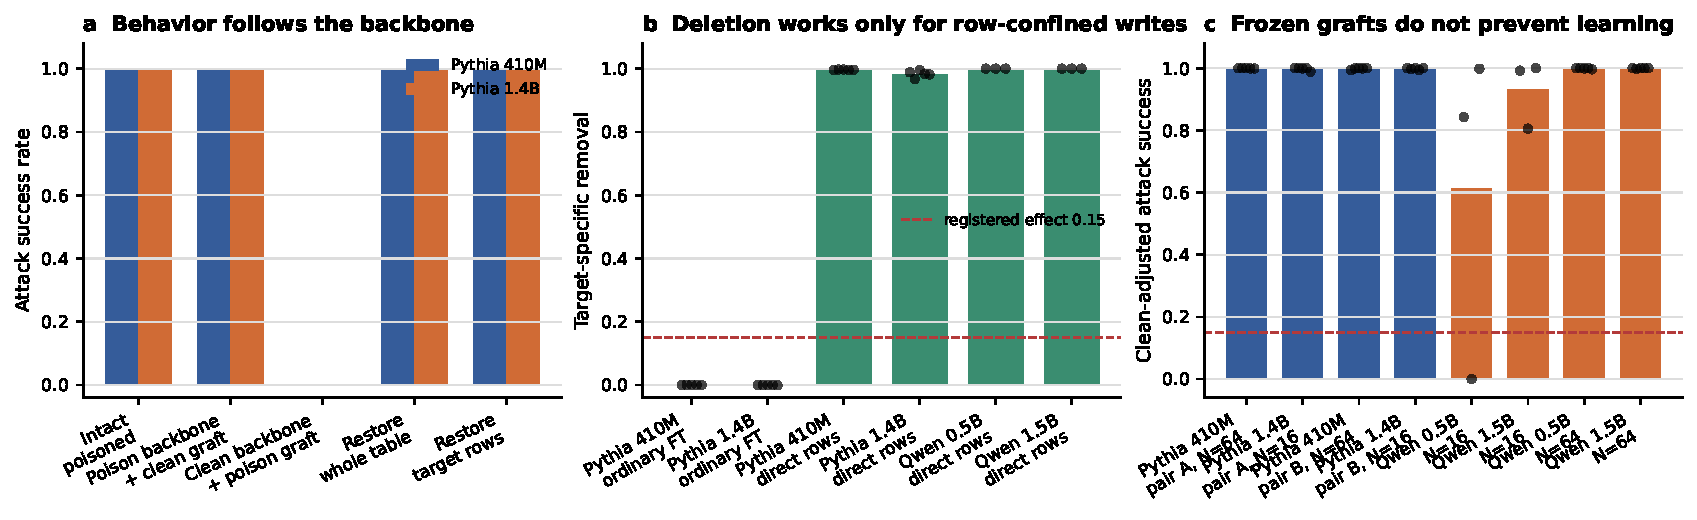
\includegraphics[width=\textwidth]{generated/core_result.pdf}
  \caption{\textbf{Deterministic addresses expose a deletion boundary, but
  ordinary fine-tuning bypasses it.} Dots are independent training seeds.
  (a) Whole-component swaps in Pythia: behavior follows the poisoned backbone,
  not the poisoned graft. (b) Target-row deletion has a null effect after
  ordinary fine-tuning but removes direct row-confined writes in Pythia and
  Qwen. (c) With the complete graft frozen, both backbone families learn the
  mapping. Qwen-0.5B at $N=16$ is the preserved reliability negative; its
  separately preregistered $N=64$ successor passes. Dashed red lines mark the
  registered meaningful effect.}
  \label{fig:core}
\end{figure*}

\subsection{Ordinary fine-tuning does not localize behavior to target rows}

Both Pythia sizes learn the primary trigger nearly perfectly with a trainable
graft. Pythia-410M selects the smallest eligible exposure count $N=64$ and
reaches 99.73\% mean ASR; Pythia-1.4B selects $N=16$ and reaches 99.55\%.
Nevertheless, target-row deletion is indistinguishable from the row controls.
Mean target-specific removal is 0.00038 with 95\% CI
$[-0.00027,0.00102]$ at 410M and $-0.00020$
$[-0.00074,0.00035]$ at 1.4B. The upper endpoints are below 0.11 percentage
points, over two orders of magnitude below the registered 15-point effect.

Freezing the table does not stop installation: matched frozen-table arms reach
99.96\% and 99.75\% mean ASR. Near-trigger hits are zero in every decisive
checkpoint; the untriggered rate is zero at 1.4B and at most 1/1,024 at 410M.
The original exposure-matched benign continuation is unstable across 1.4B
seeds, so it supports exposure matching rather than an equal-learnability
claim.

\subsection{Whole-component swaps locate the behavior in the backbone}

Figure~\ref{fig:core}a reports symmetric hybrid interventions on the same ten
Pythia checkpoints. Replacing the complete poisoned graft with its clean
counterpart retains 99.65\% ASR at 410M and 99.49\% at 1.4B. Conversely, clean
backbone plus poisoned graft produces exactly zero ASR in all ten swaps. The
mean outside-graft sufficiency contrasts are 0.9965
$[0.9912,1.0018]$ and 0.9949 $[0.9862,1.0036]$. Restoring the whole table or
only $R(z)$ changes ASR by at most 0.02 percentage points on average.

The context gate does not explain the null. Poison-minus-clean trigger-gate
shifts are 0.0332 $[-0.0753,0.1418]$ at 410M and 0.0063
$[-0.0252,0.0379]$ at 1.4B, with seed-level intervals spanning zero. Prompt
values are not treated as independent replicates.

\subsection{The deletion assay works for row-confined storage}

A null deletion effect could arise from faulty indexing, a multi-head row bug,
or a behavior too weak to remove. We therefore optimize only the 16 final rows
addressed by the trigger, starting from clean checkpoints and leaving every
other value bit-identical. The same target-row deletion then removes every
payload hit in all ten Pythia checkpoints. Target-specific removal is 0.99628
$[0.99523,0.99732]$ at 410M and 0.98301 $[0.96999,0.99603]$ at 1.4B. Benign-row
and random-row deletions are inert apart from one 0.02-point random effect.

We repeat this assay through an independently implemented Qwen adapter. Three
seeds per size reach 100\% intact ASR and 0\% after target deletion, with
target-specific removal exactly 1.0. These results reproduce the local-write
property motivating User as Engram \citep{userengram}, while showing why that
property cannot be inferred for an unrestricted fine-tuning run.

\subsection{Backbone routing transfers across families, with a dose boundary}

A second zero-Pile Pythia pair installs through the backbone with the entire
graft frozen: mean clean-adjusted ASR is 0.99844
$[0.99539,1.00148]$ at 410M ($N=64$) and 0.99824
$[0.99499,1.00150]$ at 1.4B ($N=16$). A frozen verifier is bit-exact at 410M.
At 1.4B its BF16 training trace differs, but a disclosed diagnostic replay
preserves the trigger decision while matched-benign accuracy varies. We do not
use the unstable benign result.

Qwen supplies a second architecture and tokenizer family. At the smallest
selected dose, $N=16$, Qwen2.5-1.5B passes (mean 0.933, 95\% CI
$[0.659,1.206]$), while Qwen2.5-0.5B fails because its three seeds yield 0.843,
0, and 0.998. This is a valid cross-scale negative at $N=16$. A separately
preregistered fixed-$N=64$ experiment with five new seeds then passes at both
sizes: 0.99902 $[0.99692,1.00112]$ at 0.5B and 0.99961
$[0.99852,1.00069]$ at 1.5B. All untriggered rates are zero.

The stronger dose has a specificity cost in one run: one 0.5B seed emits the
payload on 140/1,024 one-character near-trigger contexts; the other nine runs
emit none. The trigger and perturbation share four initial Qwen tokens and
diverge over the final three. This observation motivates a prospective study
of token-overlap generalization, but the present evidence does not establish
its mechanism.

\section{Related work and novelty boundary}

Engram frames deterministic conditional memory as a capacity and systems
primitive and studies scaling, reasoning, and attention allocation
\citep{engram}. Memory Grafting constructs the table offline from pretrained
hidden states and evaluates language-model quality \citep{grafting}; TF-Engram
targets train-free construction and storage hierarchy \citep{tfengram}. These
works do not test whether later unrestricted fine-tuning stores new conditional
behavior inside the addressable component.

User as Engram is the closest work \citep{userengram}. It surgically inserts
facts into known hash rows and demonstrates exact locality, composition, and
personalization. Our direct-write positive control overlaps that mechanism and
is presented as validation, not novelty. Our question is its missing converse:
given an available local store, does ordinary learning use it? The component
swaps and frozen-graft experiments show that the answer can be no.

Model editing treats transformer MLPs as implicit key--value memories and
changes localized weights \citep{rome,memit}; BadEdit uses editing to install
backdoors efficiently \citep{badedit}. That line intervenes on dense
parameters. We instead ask whether an explicit, externally addressable memory
contains behavior learned under unrestricted optimization. Agent memory
poisoning attacks corrupt retrieved natural-language records
\citep{memorypoison}; our table is a parametric hidden-state module and our
threat is training-time route ambiguity. Sleeper-agent work studies persistence
through later safety training \citep{sleeper}; we study storage location and a
specific deletion interface.

\section{Implications and limitations}

\paragraph{A write policy is part of the security boundary.}
Deterministic lookup answers \emph{where an input reads}; it does not answer
\emph{where an optimizer writes}. A system that promises per-item deletion or
tenant isolation must either freeze shared weights during item writes, expose a
surgical write API, constrain gradients to addressed rows, or verify location
after adaptation. Merely adding a table cannot provide that guarantee.

\paragraph{Synthetic behavior.}
Rare strings and one-token payloads yield precise causal assays, but they are
not realistic harmful actions, personal facts, or long-form policies. We show a
storage failure mode, not its prevalence or severity in deployment. Semantic
payloads could recruit different circuits and need separate experiments.

\paragraph{Implementation and scale.}
We test one faithful Memory Grafting implementation inserted into four base LMs
from 0.5B to 1.5B dense parameters. These are small by current deployment
standards and are not official pretrained Engram checkpoints. We do not claim
that every conditional memory, optimizer, insertion layer, or pretraining
regime routes behavior identically.

\paragraph{Optimization comparison.}
Our table-only ordinary recipe fails to install either continuation even at
$N=4096$, whereas row-restricted direct optimization succeeds with a larger
learning rate. This is itself evidence that parameterization and recipe decide
the route, but it is not a matched optimizer-efficiency comparison. Developing
a standard fine-tuning rule that both uses the table and preserves downstream
quality remains open.

\paragraph{Numerical replay.}
All registered conclusions reproduce under full replay. Some 1.4B BF16 runs do
not reproduce every non-primary argmax or loss value. We therefore claim
decision reproducibility and publish disagreement counts, rather than claiming
universal bitwise determinism.

\section{Conclusion}

An addressable memory row can be deleted exactly, and behavior confined to it
disappears. That fact does not make a model's learned behavior addressable.
Across the tested Pythia and Qwen Memory Grafts, ordinary causal-LM fine-tuning
reliably learns rare trigger mappings in the dense backbone, surviving deletion
of the trigger rows and replacement of the entire graft. Conditional memory can
support a security boundary, but only when the write path enforces it.

\bibliography{references}
\bibliographystyle{iclr2027_conference}

\appendix
\section{Evidence classification and protocol history}

Table~\ref{tab:evidence} prevents developmental and invalid attempts from being
silently promoted into evidence.
\begin{table}[h]
\centering\small
\begin{tabularx}{\linewidth}{lX}
\toprule
Stage & Classification and licensed conclusion \\
\midrule
S1 v1.1 & Valid negative for row localization; valid positive for attack installation. \\
S2a & Developmental negative: table-only ordinary recipe did not install; deletion untested there. \\
S2b--d & Valid component localization, gate measurement, and clean-NLL benign matching. \\
S2e & Valid positive control for deletion of deliberately row-confined behavior. \\
G1 & Valid second-pair Pythia result; frozen verifier failed bitwise at 1.4B, decision survived disclosed diagnostic replay. \\
G2 & Invalid before scientific training: Qwen payload tokenized to two tokens. \\
G2.1 & Invalid before marker-dependent optimizer work: local symbol shadowed the training function. \\
G2.2 & Valid Qwen surgical controls; valid $N=16$ positive at 1.5B and reliability negative at 0.5B. Assembly-only three-seed helper repair disclosed. \\
G2.3 & Valid, fully replayed fixed-$N=64$ five-seed positive at both Qwen sizes. \\
\bottomrule
\end{tabularx}
\caption{Audit classification. Invalid runs are preserved but support no
scientific claim. Development observations do not enter decisive estimates.}
\label{tab:evidence}
\end{table}

\section{Detailed model and memory configuration}

Pythia uses immutable revisions of the 410M, 1.4B, and 2.8B base checkpoints.
Qwen uses revisions \texttt{060db6499f32faf8b98477b0a26969ef7d8b9987}
(0.5B) and \texttt{8faed761d45a263340a0528343f099c05c9a4323}
(1.5B). The exact bank retains 10,000 entries for each order 2--4. Hash misses
use orders 2 and 3, eight heads per order, fixed prime table sizes, deterministic
multiplicative-XOR hashing, and a frozen textual compression map. The graft is
inserted before recipient decoder layer 1. All clean and poison partitions use
disjoint context-order seeds.

\section{Additional controls}

The Pile marker audit uses an indexed corpus rather than sampling and records
zero exact occurrences for trigger, near trigger, and benign marker strings.
Clean-checkpoint ASR is subtracted from installed ASR. Random-row controls
match the number of deleted rows. Benign-row controls address a marker with the
same number of training exposures. Later benign continuations are chosen by a
deterministic search over round-tripping one-token lowercase words to minimize
summed squared clean mean-NLL gap across both sizes. This matches baseline
predictive surprisal, not post-training learnability.

\section{Reproducibility record}

The compact plotted evidence is in \texttt{generated/EVIDENCE.json}; it records
the path and SHA-256 digest of each local source aggregate. The scientific
stages retain per-prompt JSONL predictions, per-step training logs, immutable
receipts, source and output manifests, model revisions, and verification
reports. The G2.3 scientific manifest has 33 entries and validates without a
mismatch. Its verifier inventory digest is
\texttt{1cc1310b754a2f1f9bda46ab5adc6582056be0b4c38bb29e14789217e9d497bb}.
Across the executed and replayed memory study, conservative instance allocation
is approximately 5.67 GPU-hours on one RTX PRO 6000 Blackwell Server Edition.

\end{document}
